\section{Networking}

A lot more information can be found here: \href{http://cnp3book.info.ucl.ac.be/}{http://cnp3book.info.ucl.ac.be/}

\subsection{Protocols}


\subsubsection{Layer 1: Physical}

\begin{itemize}
    \item Synchronous serial protocols: Master-slave relationship. Can only go one-way
        \begin{itemize}
            \item I2C/TWI
            \item SPI
        \end{itemize}
    \item Asynchronous serial protocols: 
        \begin{itemize}
            \item TTL Serial
            \item RS-232: your monitor cable 
        \end{itemize}
    \item Asynchronous serial bus protocols: 
        \begin{itemize}
            \item usb
            \item RS-485
        \end{itemize}
\end{itemize}

\subsubsection{Layer 2 : Data link}

\paragraph{Ethernet [Frames]} 

Ethernet is barely a protocol. It works like morse: the sender writes the destination-mac on the frame and sends it out on the wire. On the wire, the frame is broadcasted to absolutely everyone, and every computer has to check for itself if the frame was meant for it or for someone else. 

Because that is way too much work with several millions of computers in the world, we have switches. They connect two nets of computers, and if a destination-mac is on the other net, they allow the frame to be broadcast to all computers in both nets; otherwise they block the frame, which makes it only broadcast to its source-net. (Hubs are even simpler devices: they always broadcast to all nets, never even reading the destination-mac.)

Because in the 70's hubs and switches didn't have very much memory, the payload of a frame is limited to 1500 bytes. As a consequence, IP's payload is 1480 bytes, and TCP's payload is 140 bytes.

There are few problems that can arise witch switches, since they are such simple components. The one you should know about is a broadcast-storm (aka switching loop). This is where multiple switches keep broadcasting each other in search of a particular node. This can really only happen when there is a circle between switches. 

When traversing through the net, routers change the destination-mac to that of the next router on the way to the destination-ip.

\paragraph{Spanning tree protocol} is how ...

\subsubsection{Layer 3 : Network}

\paragraph{IP} 

IP is being sent in packages. Each contains the source- and destination-IP and the payload.

Ip packages are routed by routers. A router looks at the destination-ip and finds the next router that is closer to the ip. Then it changes the destination-mac to that of the next router and sends the package on its way.

IP doesn't have a notion of a connection. You can blindly send thousends of IP-packages into the ether and never know if they arrived. 

\paragraph{Discovering a router and obtaining an ip} The computer uses DHCP to find a router: it requests an IP address by broadcasting a DHCPDiscover message to the local subnet. The router hosts a DHCP server that then sends the computer an answer containing the computers new ip-adress and the default-gateway that it should use. 

\begin{lstlisting}
michael@michael-ThinkPad-Edge-E540:~$ sudo tcpdump -vnes0 -i wlp4s0 port 67 or port 68
tcpdump: listening on wlp4s0, link-type EN10MB (Ethernet), capture size 262144 bytes
13:53:33.023390 0c:8b:fd:8f:8d:65 > ff:ff:ff:ff:ff:ff, ethertype IPv4 (0x0800), length 342: (tos 0x10, ttl 128, id 0, offset 0, flags [none], proto UDP (17), length 328)
    0.0.0.0.68 > 255.255.255.255.67: BOOTP/DHCP, Request from 0c:8b:fd:8f:8d:65, length 300, xid 0x83aa8a15, Flags [none]
	  Client-Ethernet-Address 0c:8b:fd:8f:8d:65
	  Vendor-rfc1048 Extensions
	    Magic Cookie 0x63825363
	    DHCP-Message Option 53, length 1: Request
	    Requested-IP Option 50, length 4: 192.168.1.178
	    Hostname Option 12, length 26: "michael-ThinkPad-Edge-E540"
	    Parameter-Request Option 55, length 18: 
	      Subnet-Mask, BR, Time-Zone, Default-Gateway
	      Domain-Name, Domain-Name-Server, Option 119, Hostname
	      Netbios-Name-Server, Netbios-Scope, MTU, Classless-Static-Route
	      NTP, Classless-Static-Route, Classless-Static-Route-Microsoft, Static-Route
	      Option 252, NTP
13:53:33.753685 e8:37:7a:39:ed:2e > 0c:8b:fd:8f:8d:65, ethertype IPv4 (0x0800), length 346: (tos 0x0, ttl 64, id 0, offset 0, flags [none], proto UDP (17), length 332)
    192.168.1.1.67 > 192.168.1.178.68: BOOTP/DHCP, Reply, length 304, xid 0x83aa8a15, Flags [none]
	  Your-IP 192.168.1.178
	  Client-Ethernet-Address 0c:8b:fd:8f:8d:65
	  Vendor-rfc1048 Extensions
	    Magic Cookie 0x63825363
	    DHCP-Message Option 53, length 1: ACK
	    Server-ID Option 54, length 4: 192.168.1.1
	    RN Option 58, length 4: 302400
	    RB Option 59, length 4: 529200
	    Lease-Time Option 51, length 4: 604800
	    Subnet-Mask Option 1, length 4: 255.255.255.0
	    Default-Gateway Option 3, length 4: 192.168.1.1
	    Domain-Name-Server Option 6, length 4: 192.168.1.1
	    Domain-Name Option 15, length 9: "rheingold"
	    BR Option 28, length 4: 192.168.1.255
\end{lstlisting}

The 4 packets to a successful DHCP:
\begin{itemize}
    \item DISCOVER: Client connects to the network and sends out a broadcast discovery looking for its DHCP information.
    \item OFFER: The server offers the DHCP information to the client
    \item REQUEST: The client requests verification of the DHCP information
    \item ACK: The server acknowledges the DHCP request
\end{itemize}

Sometimes you will not see the DISCOVER / OFFER and just see the REQUEST / ACK. This happens when the client has already obtained a valid DHCP lease earlier and is just requesting to have it again before its lease time expires. Typically this is performed when half the lease has lapsed.

If the REQUEST is not valid anymore the server will send a NACK indicating to the client that it can no longer use this DHCP information. This should cause the client to start over with a DISCOVER.

Sometimes you will see repeated DISCOVER / OFFER but never a REQUEST from the client. This happens when the client either doesn't receive the OFFER or doesn't like it for some reason. Perhaps a firewall is blocking it, they have a poor connection, or simply they're using a Windows computer.

It's common for Windows Vista to never even start its DHCP process. It will just refuse to DISCOVER and complain that the connection is "limited or no connectivity".  You can try to diagnose the problem and tell it to reset the network card and/or get new IP information. If this fails to start it then I find adding a static IP and then setting it back to DHCP will get it going. You may even need to restart the DHCPC service. Its Vista.. where you expecting it to work as advertised?


\paragraph{Routers} are the hardware components that ....


\subsubsection{Layer 4 : Transport}

Transport-layer protocols contain Contain source- and destination-port-number. This way, a package that has already arrived at a server (by its ip-address) can be sent to the right application to handle the request. 

Common port numbers on the receiving site are:
\begin{itemize}
\item 21: ftp
\item 22: ssh
\item 25: smtp
\item 53: dns
\item 67/68: dhcp
\item 110: pop
\item 80: http
\item 443: https (http in tls)
\item 989/990: sftp (ftp in tls or ssh)
\end{itemize}

The port number only gets important once a package arrives at the destination-server. 
There, it must fist pass the firewall. Then, the server decides what application should receive packages addressed to the given port. 

\paragraph{TCP} 

Continuous connection. The recipient regularly sends the sender an ACK with the last received package number. 
If the sender receives ACKs of the last sent package, it gradually increases the ammount of packages it sends in a batch before waiting for another ACK. 
If the sender receives an ACK of the same package number multiple times, it assumes that all the following packages have been lost and retransmits them from there. Also, the batch-size is temporarily reduced. 

\paragraph{UDP}

\subsubsection{Layer 5: Application layer}

\paragraph{HTTP} 

Http kind of throws away the continuous connection created using tcp by terminating said connection once a request and all its subsequent subrequests (like fetching the image on a site) has been served. 

Http requests consist of 
\begin{itemize}
    \item a url, 
    \item a method, 
    \item and potentially parameters
\end{itemize} 

Http-resonses consist of 
\begin{itemize}
    \item a status-code, 
    \item a mime-type (= Content-type) 
    \item and the actual content. 
\end{itemize}
    
It's good to know a few of these status codes: 
\begin{itemize}
    \item 200 : all ok
    \item 302 : item was already cached
    \item 404 : resource not found
    \item 500 : internal server error
\end{itemize}

Http is really a stupid protocol. But for static websites it's just about enough. Also, webservices send and reciive their xml over http.

\paragraph{HTTPS} 

This is http within ssl (aka tls). This is not the same as http within ssh - that would be called a tunnel. ssl (port 443) and ssh (port 21) both use Diffie-Hellmann to create a common key. But the difference is that ssl does not usually require authentication of the client. The server proves its identity by sending the client a certificate, but the client does not need to authenticate to the server like he does in ssh (by password or by by public-key authentication).

In https, all the http-content, being url, headers and parameters, is encrypted. However, ip- and tcp-headers are not encrypted - otherwise the packages would not be routable. Also, for making the initial handshake with the server, the servers url has to pass through the net in public. But once https is established, clicks on further hyperlinks on the server will not be visible to the outside; only the associated ip and port.

\paragraph{Websocket}
Contrary to http, which is just a request-response-close protocol, in websockets a server has the option to query the client actively at any time. 


\subsubsection{Layer 6 and higher}

\paragraph{REST} 

REST sits on top of HTTP. It defines a few methods: 
\begin{itemize}
    \item GET: Get a ressource. Get puts all its parameters right in the url and has no body
    \item POST: Put enclosed data in database, changing an existing resource. Post-Parameters are put in the request body.
    \item PUT: Put enclosed data in database, adding a new resource
    \item HEAD: 
\end{itemize}

\paragraph{SOAP} Simple Object Access Protocol







\subsection{Email}

Ok, so we've covered the ethernet/ip/tcp/etc stack. Email is an altogether different beast. 

\paragraph{SMTP}: per default on port 25 (or 465 for TLS). For sending email.
\paragraph{POP3}: per default on port 110 (or 995 for TLS). For pulling email from server. 
\paragraph{IMAP}: per default on port 143 (or 993 for TLS). For copying email from server and syncing read-status.







\subsection{Security}

\subsubsection{Encryption}



\subsection{Making things talk: Remote data transmission}

Before we go into details, we need to know some basics of communication.

How radio works
\begin{itemize}
    \item Radio waves are the longest and contain the least energy of any electromagnetic wave. While ligthwaves are the size of bacteria, radiowaves are the size of a car of even a mountain.
    \item AM-Radio (amplitude-modulation); the original standard. 
        \begin{itemize}
            \item Take a signal of constant amplitude and frequency - know as the carrier wave. 
            \item Add your music to that signal. Even though the music has changing freqs and amps, the carrier signal transports it at its carrying frequency.
            \item Send the signal from a radio-station
            \item Receive the signal with a radio, where you pick the channel by chosing the carrier-frequency. The radio then subtracts the carrier-signal, leaving only the original music intact. 
        \end{itemize}
        This is how a signal can be transmitted on one single frequency. 
    \item FM-Radio does the same, but instead of staying on one freq and listening to amplitude, it listens to a (small) spectrum of freqs and emmits sound whenever the frequency changes. 
        \begin{itemize}
            \item better against interference, because intf often causes ampl spikes
            \item smaller range: AM can transmit over long distance because it uses a smaller frequency (though not so good quality)
        \end{itemize}
    \item in modems, isdn and dsl we use am, fm and phase-modulation together to allow for multiple channels. 
\end{itemize}



Types of wires.
\begin{itemize}
    \item copper: traditional telephone wires. ISDN runs on these; DSL does too, but somewhat slower (this is because, contrary to ISDN, DSL needs an IP-Station as soon as possible after leaving your house. In rural areas DSL becomes much slower this way). Can carry electricity, which is why in the past telephones still worked even when a houses electricity crashed. 
    \item glass-fibre/voip: old copper wires are being replaced with cables that end in a station with IP-adress. These don't carry electricity anymore, however. ISDN does not work on these, either. Those new voip-cables are often glass-fibre cables\footnote{Instead of electricity, glass-fibre cables carry light-signals. This technology allows for far more frequency bands to be used.}. DSL over glass-fibres is called VDSL (whereas DSL on the old copper wires is simply called DSL), telephony over DSL/glass is called VOIP.
\end{itemize}

And here a recap on important hardware: 
\begin{itemize}
    \item Router: really consists of three devices: 
        \begin{itemize} 
            \item router: sends packets by ip either to your devices or the next router on the internet
            \item switch: broadcasts incomming packets to all your home-devices or moves outgoing packets to the router
            \item wireless access point
        \end{itemize}
\end{itemize}

\subsubsection{ISDN (wired)}
Your computer is attached to a modem\footnote{modem stands for modulator/demodulator: a device which receives electrical waves comming from the copper-wire and transforms them into analog (sound) or digital (bits) waves; and back.}, which is attached to a telephone-cable or even a telephone-earpiece (!). The modem translates your TCP-requests to sound-signals which would be carried over the telephone-wire in the form of sound. With ISDN, you cannot use both your telephone and your internet at the same time (actually, with am, fm and pm you can; you'd obtain up to 3 channels).  
Actually, isdn is different from a modem. Modems came first. There you put your telephone directly on the earpiece. Isdn then skipped the earpiece and put the modem directly onto the copper wire - this way a higher sampling frequency was possible. 
Since everyone in a neighbourhood shares the same cable, your speed will drop when many people use netflix at the same time. 
On the other hand, ISDN uses a boosting technology that makes sure that your phone-conversation stays clear over large distances. This means that ISDN does not require a relay nearby - contrary to DSL. So in rural areas, ISDN may be actually faster. 
Speed: around 0.1 Mbit/s.


\subsection{DSL (wired)}
DSL (digital subscriber line) is using ordinary telephone wires or the more modern glass-wires (in that case it is called VDSL). Both a telephone-cable as well as a your routers output will be plugged into a DSL-splitter (shown below).
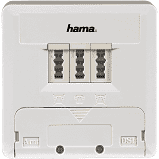
\includegraphics{images/dsl_splitter.png}
With ISDN, you could not use your telephone and your computer at the same time. This is because your internet-traffic is going through the copper-wire on a different frequency-band than the one telephone-conversations use.  
ISDN was hampered by interference, because multiple wires would lie in the ground close to each other. While ISDN did already use am, fm and pm, DSL has a technique for interference-cancelling that allows it to increase its throughput even more. But this technology requires an ip-station at the end of the line. 
To further increase speed for the average user, there is \emph{A}DSL, with A standing for asymetric. Here, downstream traffic is much prefered to upstream, since the average user does not host a server.
Contrary to ISDN, DSL connections are not shared between all users in a neighbourhood. Instead, a dedicated connection runs directly to a station with its own IP-adress near your house. 
Speed: up to 16 Mbit/s, but only 1-2 Mbit/s in rural areas where IP-Stations are far from your house.


\subsection{WiFi (really only those few meters up to your wired router)}
WiFi really uses the same "everyone-shout-first-gets-served" protocol as MAC does. That means that every device has to wait its turn to use the router. 
There are two frequencies at which devices may communicate:
\begin{itemize}
    \item 2.4 GHz: slower, further reach
    \item 5.0 Ghz: faster, but only at shorter distance
\end{itemize}


\subsection{GSM, EDGE, 3G=HSDPA, 4G=LTE=HSDPA(+) (radio)}
When your device has no WLAN or LAN access to a router, you can only access the internet by going over radio-stations (or satellite, see later). 


\subsection{GPS (satellite)}
Since with GPS a signal has to travel all the way to space and back, this is the slowest of the communication methods. 